\documentclass[citation\_needed]{subfiles}
\begin{document}

Apprendre des représentations denses des tokens permet d'améliorer grandement la qualité des modèles de réseaux de neurones. Ces représentations se basent généralement sur des analyses distributionnelles. Plus précisément, il est possible d'apprendre ces représentations sur de grands volumes de textes à l'aide de modèles de langue. Dans cette section, nous ne parlerons que des modèles de langues neuronaux car nous les appliquerons dans le cadre de réseaux de neurones. Ce processus est généralement appelé le \emph{pré-appentissage de représentations}.

Un \emph{modèle de langue} est un modèle probabiliste modélisant la probabilité d'observer une séquence de tokens dans une langue :

\begin{equation}\label{eq:language-model}
P(t_{1},...,t_{m}) = P(t_{1}) \times P(t_{2}|t_{1}) \times ... \times P(t_{m} | t_{1}, t_{2}, ..., t_{m-1})
\end{equation}

En appliquant l'hypothèse de Markov, cette probabilité peut être approximée en n'utilisant qu'un contexte de taille $n$, le modèle de langue étant alors un modèle de Markov d'ordre $n$. Ces modèles sont appelés les modèles de langues n-gramme. Un modèle de langue parmi les plus simples modélise la probabilité du token courant étant donné le token précédent \citep{bengio2003neural}. L'espace de sortie d'un modèle de langue est donc le vocabulaire $V$ tel que défini dans la section \ref{subsubsec:nn-embeddings}. L'un des logiciels les plus utilisés pour calculer ce type de représentations est word2vec \citep{mikolov2013efficient,mikolov2013distributed}, dont nous détaillerons les principaux aspects dans la suite de la section.

word2vec définit deux modèles de langues, l'un appelé \textit{continous bag of words}\footnote{traduisible par "sac de mots continu"} et l'autre appelé \textit{skip-gram}\footnote{traduisible par "saute-gramme continu"} \citep{mikolov2013efficient}. Le second étant la variante la plus utilisée et souvent celle donnant les meilleurs résultats, nous de détaillerons qu'elle ici. L'idée de ce modèle est de prédire les tokens voisins du token courant dans une fenêtre de taille fixe donnée à l'avance, $c$. Si nous avons le token $w_{t}$ à un indice t dans la séquence, l'idée est de prédire les différents tokens $\{w_{t-c},w_{t-c+1},...,w_{t-1},w_{t+1},...,w_{t+c}\}$. Une représentation graphique du modèle skip-gram est donné dans la figure \ref{fig:skipgram}. Cette modélisation est intéressante car la représentation d'un token est calculée afin de prédire au mieux les tokens aux alentours. Dans le cadre d'un outil de TAL, ces représentations sont normalement robustes à la présence de tokens inconnus.

\begin{figure}[ht!]
    \centering
    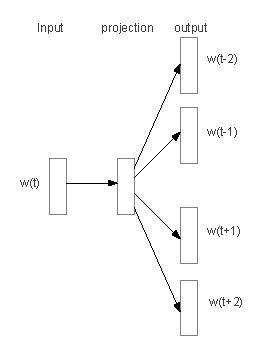
\includegraphics[scale=1.2]{images/NN/word2vec/skipgram}
    \caption{l'architecture du modèle skip-gram. Le but du modèle est d'apprendre des représentations des tokens capables de prédire efficacement les tokens voisins.}
    \label{fig:skipgram}
\end{figure}

Plus formellement, étant donné un corpus constitué d'une séquence de tokens $W = \{w_{1}, w_{2}, ..., w_{T}\}$ et leurs contextes correspondants $C = \{c_{1}, c_{2}, ..., c_{T}\}$ l'objectif du skip-gram est d'obtenir les meilleurs paramètres du modèle $\theta$ afin de maximiser la probabilité du corpus :

\begin{equation}\label{eq:skipgram}
\argmax{\theta} \prod_{1 \leq i \leq T} p(c_{i}|w_{i};\theta)
\end{equation}

Il est à noter que le but ici est plus d'avoir un bon $\theta$, donc une représentation de chaque token, capable de rapprocher et distinguer les différents tokens, plutôt que de maximiser directement la probabilité du corpus. La fonction de décision du \textit{skip-gram} est le \textit{softmax} (équation \ref{eq:softmax}) :

\begin{equation}\label{eq:skipgram-softmax}
p(c_{i}|w_{i};\theta) = \frac{e^{v_{c_{i}} \cdot v_{w_{i}}}}{\sum_{c' \in C} e^{v_{c'} \cdot c_{w_{i}}}}
\end{equation}

Où "." est le produit scalaire, $v_{c_{i}}$, $v_{w_{i}}$ et c' $\in$ $R^{d}$ des représentations denses de dimension $d$ pour $c_{i}$, $w_{i}$ et c'. La fonction objectif s'écrit alors :

\begin{equation}\label{eq:skipgram-objective}
\begin{aligned}
%  &\ \argmax{\theta} \prod_{1 \leq i \leq T} p(c_{i}|w_{i};\theta) \\
%= &\ \argmax{\theta} \prod_{1 \leq i \leq T} \frac{e^{v_{c_{i}} \cdot v_{w_{i}}}}{\sum_{c' \in C} e^{v_{c'} \cdot c_{w_{i}}}}\ selon\ \ref{eq:skipgram-softmax}\\
%= &\ \argmax{\theta}\ \log \prod_{1 \leq i \leq T} \frac{e^{v_{c_{i}} \cdot v_{w_{i}}}}{\sum_{c' \in C} e^{v_{c'} \cdot c_{w_{i}}}} \\
= &\ \argmax{\theta} \sum_{1 \leq i \leq T} \left( \log(e^{v_{c_{i}} \cdot v_{w_{i}}}) - \log \sum_{c' \in C} e^{v_{c'} \cdot c_{w_{i}}} \right) \\
\end{aligned}
\end{equation}

Lorsque la taille des contextes $C$ est grande ($>1000000$ tokens par exemple), l'utilisation de \textit{softmax} est particulièrement coûteuse car il faut sommer sur l'ensemble des contextes à chaque token du texte. Une proposition pour réduire le coût de l'apprentissage tout en gardant une approximation proche de l'objectif initial est le \textit{negative sampling} (échantillonnage négatif) \citep{mikolov2013distributed}. L'idée de cette approche est que, si le corpus est suffisamment grand, il n'est pas nécessaire d'observer l'ensemble des contextes du corpus à chaque instant. Pour chaque token, un échantillon de petite taille peut être généré de manière aléatoire. En assumant que cet échantillon soit systématiquement négatif, nous pouvons obtenir une bonne estimation de $\theta$ maintenant ses capacités de rapprochement et distinction de tokens, à condition que le corpus soit assez large.

Nous pouvons alors constuire un objectif plus simple d'un point de vu computationel. Pour cela, nous définissons d'abord $D=\{(w_{i},c_{i})| w_{i} \in W, c_{i} \in C,\ et\ 1 \leq i \leq T\}$, l'ensemble des tokens associés à leur contexte, $p(D = 1|w, c;\theta)$, la probabilité qu'un token $w$ soit observé dans un contexte $c$ selon le modèle. $p(D = 1|w, c;\theta)$ peut se définir également par le \emph{softmax}, donnant alors l'objectif :

\begin{equation}\label{eq:negative-sampling-naive}
\begin{aligned}
  &\ \argmax{\theta} \log \prod_{(w,c) \in D} p(D=1|c,w;\theta) \\
= &\ \argmax{\theta} \log \prod_{(w,c) \in D} \frac{1}{1+e^{-v_c \cdot v_{w}}} \\
= &\ \argmax{\theta} \sum_{(w,c) \in D} \log \frac{1}{1+e^{-v_c \cdot v_{w}}} \\
\end{aligned}
\end{equation}

Cette fonction objectif est triviale car le classifieur n'est alimenté que d'exemples positifs, il est possible d'ajuster $\theta$ de sorte que $p(D = 1|w, c;\theta)=1$ pour chaque paire $(w,c) \in D$. Afin d'éviter ce phénomène, une solution simple est de présenter au classifieur des exemples négatifs. De manière analogue à $D$, nous pouvons alors générer un ensemble $D'$ d'exemples négatifs où les contextes sont tirés aléatoirement. Nous pouvons alors définir $p(D=0|w,c;\theta) = 1 - p(D=1|w,c;\theta)$ la probabilité que $(w,c)$ ne soit pas observé dans les données. L'objectif devient alors :

\begin{equation}\label{eq:negative-sampling}
\begin{aligned}
  &\ \argmax{\theta} \prod_{(w,c) \in D} p(D=1|c,w;\theta) \prod_{(w,c) \in D'} p(D=0|c,w;\theta) \\
%= &\ \argmax{\theta} \prod_{(w,c) \in D} p(D=1|c,w;\theta) \prod_{(w,c) \in D'} 1 - p(D=1|c,w;\theta) \\
= &\ \argmax{\theta} \prod_{(w,c) \in D} \frac{1}{1 + e^{-v_{c}.v_{w}}} \prod_{(w,c) \in D'} 1 - \frac{1}{1 + e^{-v_{c}.v_{w}}}\ selon\ \ref{eq:negative-sampling-naive} \\
%= &\ \argmax{\theta} \prod_{(w,c) \in D} \frac{1}{1 + e^{-v_{c}.v_{w}}} \prod_{(w,c) \in D'} \frac{1 + e^{v_{c}.v_{w}}}{1 + e^{v_{c}.v_{w}}} - \frac{e^{v_{c}.v_{w}}}{1 + e^{v_{c}.v_{w}}}\ selon\ \ref{eq:sigmoid} \\
%= &\ \argmax{\theta} \log\left( \prod_{(w,c) \in D} \frac{1}{1 + e^{-v_{c}.v_{w}}} \prod_{(w,c) \in D'} \frac{1}{1 + e^{v_{c}.v_{w}}} \right)\ selon\ \ref{eq:sigmoid} \\
= &\ \argmax{\theta} \sum_{(w,c) \in D} \log \frac{1}{1 + e^{-v_{c}.v_{w}}} \sum_{(w,c) \in D'} \log \frac{1}{1 + e^{v_{c}.v_{w}}} \\
= &\ \argmax{\theta} \sum_{(w,c) \in D} \log(\sigma(v_{c}.v_{w})) \sum_{(w,c) \in D'} \log(\sigma(-v_{c}.v_{w}))\ selon\ \ref{eq:sigmoid}\\
\end{aligned}
\end{equation}

L'idée ici est qu'apprendre à distinguer des tokens positifs de tokens négatifs, même générés aléatoirement, permet d'obtenir de bonnes représentations pour les tokens. La fonction de génération aléatoire de contextes négatifs influe grandement sur les résultats. \citep{mikolov2013efficient} utilise simplement la probabilité d'un token à la puissance $3/4$, donc $\frac{count(c)}{T}^{0.75}$, même si ce choix n'est pas motivé par une raison autre que l'observation empirique de meilleurs résultats. Des exemples de tokens avec leurs plus proches voisins selon des représentations pré-apprises (avec un autre outil que word2vec) sont donnés dans le tableau \ref{tab:word-neighbours}. word2vec permet d'obtenir des représentations similaires. Ces représentations, comme dit dans la section \ref{subsubsec:nn-embeddings}, ont des propriétés analogiques intéressantes. Il a été montré notamment que $E(Paris)\ -\ E(France)\ +\ E(Italy)\ \approx\ E(Rome)$, que l'on peut lire "Rome est à l'Italie ce que Paris est à la France". Une autre équivalence était $E(roi)\ -\ E(homme)\ +\ E(femme)\ \approx\ E(reine)$.

\begin{table}[ht!]
\footnotesize
\centering
\begin{tabular}{cccccc}
FRANCE & JESUS & XBOX & REDDISH & SCRATCHED & MEGABITS \\
454 & 1973 & 6909 & 11724 & 29869 & 87025 \\
\hline
AUSTRIA & GOD & AMIGA & GREENISH & NAILED & OCTETS \\
BELGIUM & SATI & PLAYSTATION & BLUISH & SMASHED & MB/S \\
GERMANY & CHRIST & MSX & PINKISH & PUNCHED & BIT/S \\
ITALY & SATAN & IPOD & PURPLISH & POPPED & BAUD \\
GREECE & KALI & SEGA & BROWNISH & CRIMPED & CARATS \\
SWEDEN & INDRA & PSNUMBER & GREYISH & SCRAPED & KBIT/S \\
NORWAY & VISHNU & HD & GRAYISH & SCREWED & MEGAHERTZ \\
EUROPE & ANANDA & DREAMCAST & WHITISH & SECTIONED & MEGAPIXELS \\
HUNGARY & PARVATI & GEFORCE & SILVERY & SLASHED & GBIT/S \\
SWITZERLAND & GRACE & CAPCOM & YELLOWISH & RIPPED & AMPERES \\
\end{tabular}
\caption{6 tokens avec leurs 10 plus proches voisins selon des représentations apprises sur le vocabulaire des 100000 tokens les plus fréquents du Wall Street Journal. Tableau repris de \citet{collobert2011natural}}
\label{tab:word-neighbours}
\end{table}

Ces représentations précalculées sur de larges quantités de textes ont de nombreux avantages. Le premier est le caractère couvrant de ces représentations, le vocabulaire d'un large texte est en effet beaucoup plus fourni que celui d'un corpus annoté, ces représentations auront donc une meilleure qualité sur les tokens inconnus. Elles ont également l'avantage d'être réutilisables pour une grande variété de tâches, ces représentations portant des informations distributionnelles intéressantes. Un autre effet de cette propriété est que le processus d'apprentissage se retrouve accéléré, les représentations précalculées étant bien plus proche de l'optimal que des représentations qui seraient initialisées aléatoirement.

À présent que nous avons décrit comment les tokens étaient représentés pour être utilisés dans un réseau de neurones adapté aux tâches de TAL. Nous présenterons dans la section suivante l'un des premiers réseaux de neurones à utiliser des représentations denses, à savoir le réseau de neurones convolutionnel tel que présenté par \citet{collobert2008unified}.

\end{document}